\documentclass[class=article, crop=false]{standalone}
\usepackage{graphicx}
\graphicspath{{../Figures}}
\usepackage{cleveref}

\begin{document}
This project can be very broadly divided into two segments, the simulation segment and the control system segment. The goal is that the simulation is to be as true to reality as possible. With a true-to-life simulation, a control system can be built to work in the simulation. Once the control system is created and tested satisfacotrily, it can hypothetically be "transplanted" to the physical test. Because of these two different segments, I will talk about them separately.

\section{Details on the simulation setup}
The exact details of the implementation are more specifically brought up in \cite{specialization}. Below is a brief elaborate of the simulation setup, further than what was mentioned in \cref{sec:basic_sim}.

The two vessels to be simulated are the surface vessel and the ROV. The ROV was simplified as a cuboid with the proper dimensions according to the manufacturer's specifications. The ROV to be used is a modified BlueROV2 Heavy made by Blue Robotics. The dimensions of which are 575 x 254 x 457 mm (WxHxD). The density of the ROV has not been tested, but is implemented in the simulation as 2000kg/m³. This is a rough estimation and the real density is likely lower. A high density like this is chosen because the ROV is supposed to be negatively buoyant,

The surface vessel was modelled roughly in CAD and then exported as a \texttt{.obj} 3D-file for AGX to work with. The dimensions and shape of the vessel are roughly corresponding with the real vessel, though not exactly as it is- intended to be exchanged for a more detailed model produced by a different master project at a later date. The density of the surface vessel is implemented at 600kg/m³ which was arrived at by taking a rough average of the different densities of carbon fiber sandwich plate we had for building the hull and then adding some extra mass to account for batteries, sensorics and other added weights.

As a note on the densities of the vessels: while AGX is able to model non-uniform densities and varying density distributions, this was not implemented in this simulation simply for the constraint of time. It was assumed that the loss of accuracy from assuming uniform density is small enough not to matter. This will be further discussed in \cref{sec:sim_discussion}

Since the ROV sinks it needs a constant force to not sink to the bottom of the simulated ocean. This is achieved by a tether connected to the surface vessel. The tether is modelled as a non-buoyant rope/wire with a radius of 10mm and a Young's modulus of \(10^9\). These figures are all assumed values and should be corrected when the real values from the physical implementation are known.

The two vessels and the tether are placed in a 200x200x120m pool of water. It is possible in AGX to simulate different sea-states, this was a part of the development work done for this project and is discussed later.


\subsection{Improvements made since specialization project}
\label{sec:simulation_work}
In addition, the simulator now is capable of simulating the winching movement of the winch on the ROV. Previously it was implemented as a fixed length wire. This means that the crane now is able to operate. A basic controller for the crane has been created as well.

The simulation has been further developed to allow for more dynamic changing of the seastate. Originally the seastate was implmented as no sea. This is now changable by changing a single variable. The sea is simulated using the wave height equation, \cref{eq:waveheight}
\begin{equation}
\label{eq:waveheight}
h = 0.5\sin(0.5 x +0.6t) + 0.25\cos(0.6y + 0.3x + 1.45t)
\end{equation}
Where \(h\) is the height above \(z=0\), \(x\) and \(y\) are the position in the horizontal plane and \(t\) is the time since the simulation started.

All of the code for the simulations as well as for the control system is available on Github at \url{https://github.com/MagnusKjorseng/FordypOgMaster/tree/recovery/Simulator/V4} \cite{noauthor_fordypogmastersimulator_nodate}

\section{Control System}
The control system implemented in the specialization project was simply taking in the position of the vessel directly from the simulation, calculating the error from the desired position and then calculating a command based on a PID controller. This worked well enough for a proof of concept, but is difficult to work with when the project increases in scope.

One of the achieved goals of this project has been to decouple the simulation from the control system. This has been done for several reasons relating to the control of the vessels. Most relevant for this project has been a decrease in development and testing time. With the different nodes of a system decoupled, it is possible to work on each node more or less individually, connecting or disconnecting them as needed. Using the node based structure of ROS2 also makes it a lot easier to develop new nodes, as the communication between nodes is clearly defined in the topics and services the nodes communicate over.

The overall desired architecture of the new control system is shown in \cref{fig:architecture}. If translated into "ROS terms", the boxes shown are nodes while the arms connecting them are the topics they communicate via.

\begin{figure}
    \centering
    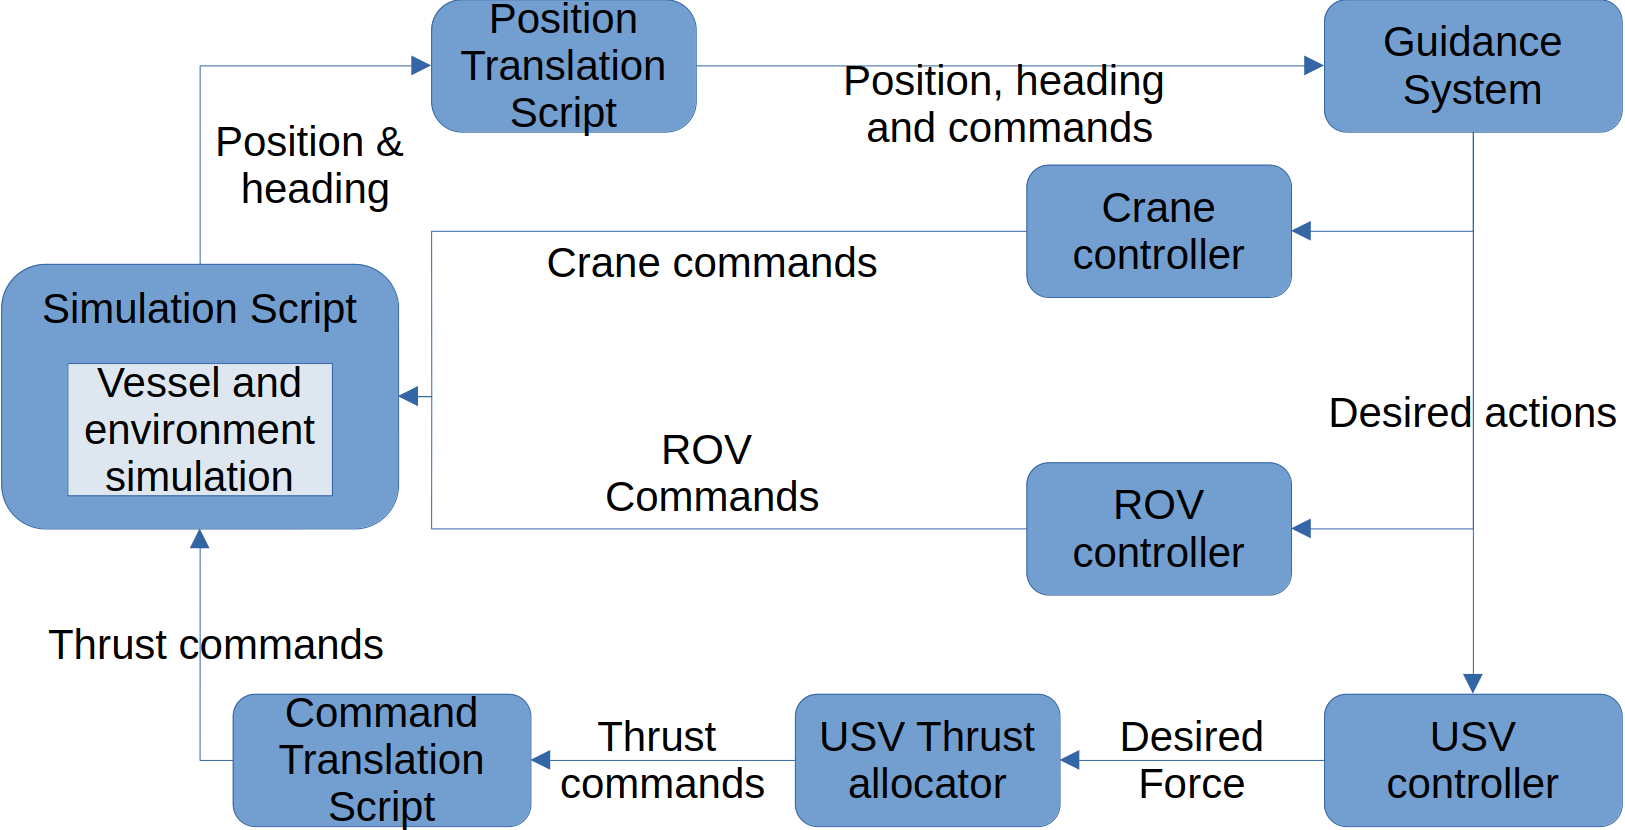
\includegraphics{control_system_graph}
    \caption{The shape of the designed control system}
    \label{fig:architecture}
\end{figure}

There are some nodes in \cref{fig:architecture} that are not as obvious at first glance, these are described further here. The "position" and "command" translation scripts exist as a middleware between the simulator and the control system. In order for the control system to be as true-to-life as possible, it has been implemented to accept position data for the USV in the form that a GPS antenna would output, so-called NMEA messages. Message types in ROS2 are strictly defined, and there exist packages which supply these NMEA messages. However, due to limitations of the simulation framework the simulator is not easily able to handle other ROS packages than the ones it has been made with, and the NMEA package is not among them. Therefore, the translation scripts work between the simulator and the control system proper. The simulation outputs position and orientation of the vessels in its own world-space, and the position translation script converts this into a lat-lon format based on a predefined baseline. This then is packaged into the correct format and sent to the guidance system. Similarly, the command translator receives the commands in a custom format and translates it into a format that the simulator can work with. In a real-world setting, these translation scripts would not be included.

The guidance system is a sort of "central controller", it is what decides the setpoints for the other controllers and instructs them. For instance, on the topic of mastering, the central controller is what would handle that. Mastering, as mentioned in the title, refers to which of the two main vessels, ROV or USV, is "in charge". Because the movements of the vessels are dependent on each other, it would not work to have them try to move in opposite directions from each other. With a more conventional neutrally buoyant ROV this might work, as the tether does not provide as firm of a link between the vessels. This is further discussed in \cite{specialization}. Ideally, this control system would be able to have either the USV or the ROV be the master, depending on the given situation. If the ROV is undertaking precision work on the seafloor, the USV should work to disturb as little as possible. If the USV needs to move while the ROV is deployed for one reason or another, the ROV should attempt to follow to not put undue strain on the wire. This is what is referred to as "reversible mastering", and the guidance system would be in charge of this. Additionally, the guidance system would handle how the crane and ROV handle vertical movement. Because of the length and elasticity of the wire, it would be a good idea to have only larger movements be taken up by the crane and allow the ROV to use its vertical thrusters to do smaller corrections. This is because due to the large length of the wire, the forces take a long time to transfer all the way down to the ROV. A lot of the movement might also be taken up as stretch in the wire and never properly reach the ROV. Because of these considerations, the crane and ROV should have different height controllers, and this is handled by the guidance system.

The last new part of the system in \cref{fig:architecture} is the USV thrust allocator. The allocator works like a translation layer between the controller and the local controllers of the USV's thrusters. The controller provides a force input on the vessel's center of gravity, but the thrusters need to know how much to thrust and in which direction. The allocator figures this out.

In abstract terms, the allocator finds and applies a transformation matrix \(T\) such that \[Tf = \tau\] where \(f\) is a vector of vectors with the lateral forces for each thruster. For this case with two thrusters, it will look something like \[f = \begin{bmatrix}x_1 \\ y_1 \\ x_2 \\ y_2 \end{bmatrix}\]
The transformation matrix can be written explicitly for the USV, since it has a very simple thrust configuration. For larger configurations it might be better to write each thruster's transformation individually and either add or remove them depending on the type of move necessary (larger moves use only larger thrusters etc.).
\begin{equation}\label{eq:transform_matrix}
T = \begin{bmatrix}1 & 0 & 1 & 0 \\ 0 & 1 & 0 & 1 \\ -l_{y_1} & l_{x_1} & -l_{y_2} & l_{x_2}\end{bmatrix}
\end{equation}

\begin{figure}
    \centering
    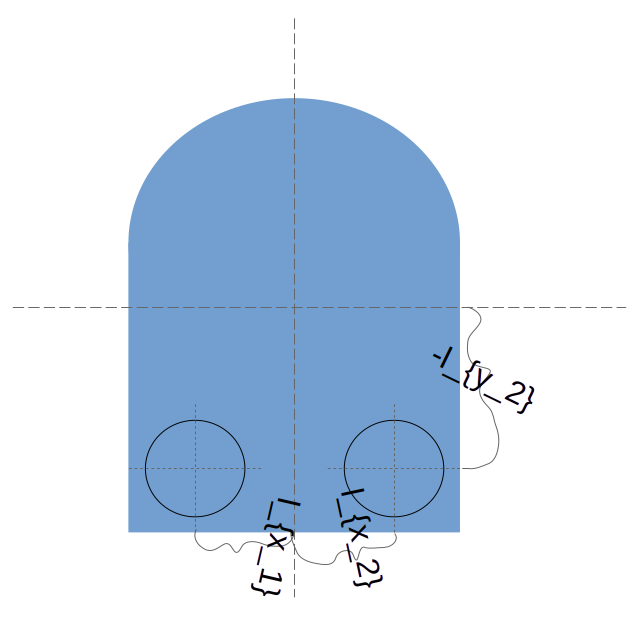
\includegraphics[width=0.9\textwidth]{thruster_position_sketch}
    \caption{Rough sketch of how the thruster position values in \cref{eq:transform_matrix} are found. The thruster configuration will be input to the allocator through a config file.}
    \label{fig:thruster_position_sketch}
\end{figure}

Since \(\tau\) and \(T\) are known, we can find \(f\) by performing a pseudoinverse on \(T\) leading us to the equation

\begin{equation}\label{eq:final_allocator}
f = T^\dagger \tau
\end{equation}

where \(T^\dagger\) is the pseudoinverse of \(T\).

This can also be written longform as

\begin{equation}\label{eq:long_allocator}
\begin{bmatrix}x_1 \\ y_1 \\ x_2 \\ y_2 \end{bmatrix} = T^\dagger \begin{bmatrix}X \\ Y \\ N\end{bmatrix}
\end{equation}

The full matrix for \(T^\dagger\) is omitted because the pseudoinverse of a non-square matrix tends to be large and ugly. Because the pseudoinverse will only ever be calculated and used by the allocator, the exact values of it are not important to know or keep track of for humans.

\section{Case description}
The USV controller implemented is quite simple. It has no predictive capability and is completely reactive. This scenario is made to compare the controller's actions as well as the error of the system in varying seastates. The simulation framework does allow for current and wind simulations as well, but these are not implemented and thus will not be simulated. The goal for the surface vessel is to stay stationary, simulating an operation where dynamic positioning is necessary for the ROV to do its work. Additionally the ROV will attempt to follow the movements of the USV so as not to put undue tension on the tether.

Five cases will be compared here, from 0m wave height to 2m wave height, in increments of 0.5m. The different kinds of seas are simulated with the same wavelength. The wave simulation is a simple regular wave in two dimensions with its wave height defined by the equation \cref{eq:waveheight}. The equation was taken from Algoryx's examples for buoyancy simulation for simplicity and ease of use. The actual value of the equation is irrelevant in the larger scheme of things because the only thing it's doing is providing a local height offset. This offset will then be used to determine how far from the zero-height of the world the vessel is. This equation has been deemed to be "random enough" for the control system to get some challenges. Further discussion around using a regular seastate is done in \cref{sec:sea_discussion}


The expected response assuming a well functioning system is that the error should be relatively minor, but there is the danger of the seas being too high. If the seas are two high there are two potential faults, the surface vessel might capsize or the thrusters might exceed their authority. The first fault is obviously disastrous and should be avoided at all costs. The second is unfortunate and might lead to loss of control or scrubbing of the mission. Both of these faults can be used as limits to find the maximum acceptable operational criteria for a mission.
\end{document}











\section{Physical setup}
\subsection{Surface vessel}
The Plan Sea project was contacted by the shipyard Brødrene Aa, in Hyen, Norway, and asked if they wanted an introduction to composite hull construction and some free materials. The Plan Sea project accepted this and got training and materials in how to apply and build a vessel from carbon fiber sandwich boards.

The sandwich boards are built up of a central foam core clad with 3-5 layers of carbon fiber weave and epoxy. Using the foam core it is possible to achieve stronger hulls than using the carbon fiber alone would, while also being lighter than an equivalent strength hull made from only carbon fiber.

The vessel was constructed as a two-engine catamaran with rough dimensions of 2.5x2x1m. A catamaran construction was chosen due to the small size of the vessel not affording a lot of stability, a catamaran would allow for a wider hull without significantly increasing hull drag compared to a monohull construction.

Another bonus of having a catamaran construction as opposed to a monohull construction is that by simply cutting a hole in the deck between the hulls, a "moonpool" is achieved. This lets the ROV be lifted at a point closer to the center of mass for the catamaran which leads to fewer instabilities in the system and less chance of capsizing or other catastrophe.

The thrusters for the surface vessel have been made using two Torqeedo Cruise 3FP thrusters. The thrusters are fully electric and designed for through-hull mounting. This makes the modification from stationary to azimuth thrusters relatively simple. The modified azimuth thrusters were mounted to the aft of the two hulls, one in each. If this is too little thrust it is possible to mount further thrusters further forward to provide assistance, either for propulsion, DP or redundancy.


\subsection{Subsea vessel}
The subsea vessel is based on a BlueROV2 Heavy, made by BlueRobotics. The BlueROV is a prosumer-grade battery operated remotely operated vehicle. It's approximately 0.5x0.5x0.3m in WxDxH. The ROV has been acquired to use for the Plan Sea project specifically. It is not the ideal solution for this case, but it's been decided that modifying an existing and functioning solution is better than attempting to build a new one, at least for this proof of concept.

A bracket has been designed to account for a mounting point for the USBL transponder, as well as to securely mount to the ROV already in use.

\subsection{Crane}
A crane needs to be designed. Thsi can be done as simply as possible having just a simple A-frame crane mounted over a moon pool. The crane system needs to consist of a few different parts. The gantry/frame itself, a winch motor, a winching system for the ROV tether and a winching system for the ROV lifting wire.
\subsection{Control systems/Ancillary}
the entirety of the control system will be acting as one big system divided into many smaller parts. The fact that ROS allows for multiple subscribers and publishers to various topics means that each element can have its own local controller that only interacts with the others. This means that the surface vessel, the crane and the ROV will all act as independent parties in the same system.
\subsubsection{ROV control}
The ROV's control system is based on an ArduPilot implementation. ArduPilot is an open-source autopilot system which is intended to be used for any remote or unmanned vehicle. The current implementation needs to be modified to allow for the type of control that's required for the project.

The majority of heave-movement will be caused by the crane onboard the surface vessel, rather than the thursters on the ROV as it's set up for by default.

\begin{figure}
    \centering
    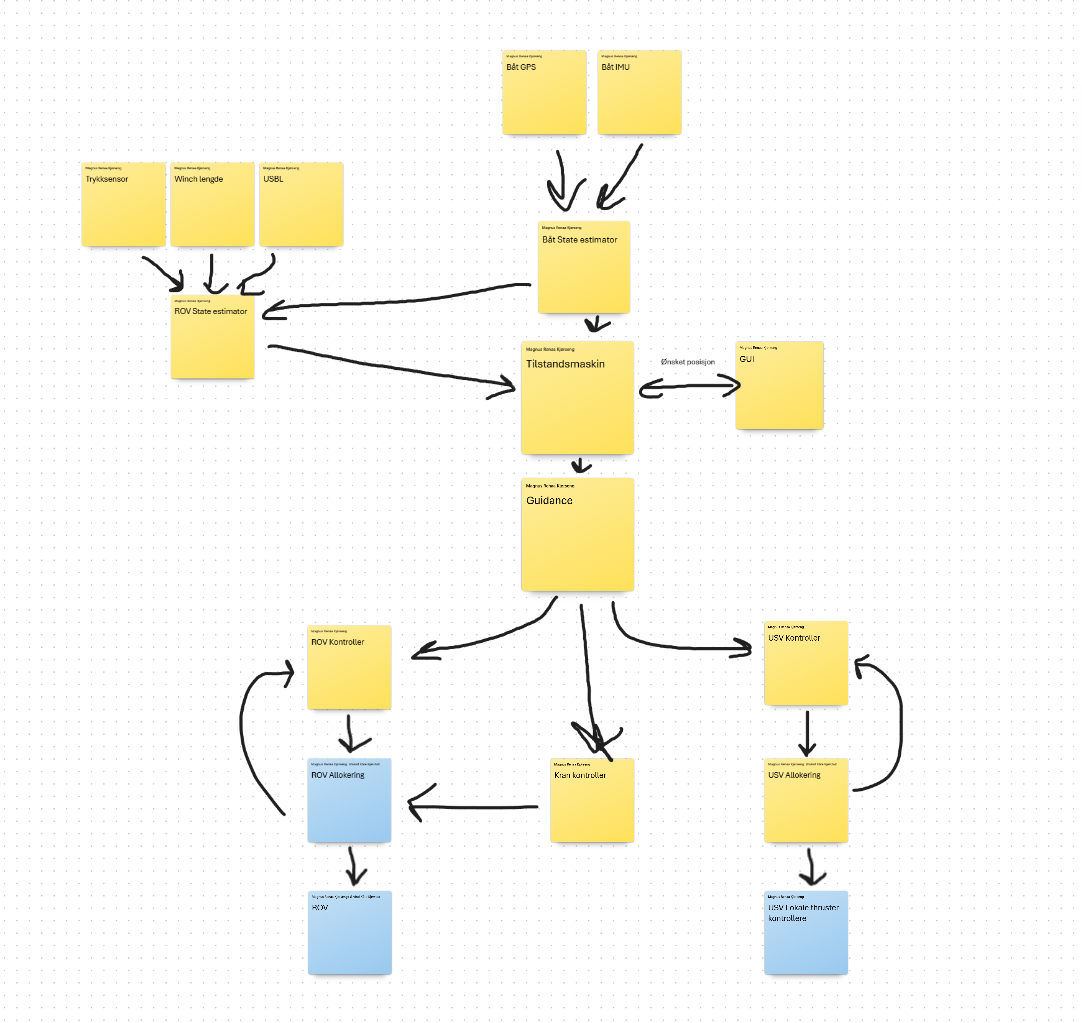
\includegraphics[width=0.9\textwidth]{control-system}
    \caption{A sketch of the control system design. TODO: Fiks bedre illustrasjon}
    \label{fig:control-system}
\end{figure}

\section{Sensorics}
The first step to knowing where to go is knowing where you are.

There are several pieces of sensorics that will be used for positioning of the system.

\subsection{GNSS}
Firstly, Global Navigational Satellite Systems, or GNSS, will be used to position the USV. There are several separate systems for GNSS, including GPS, Gallileo and GLONASS to mention a few.

The exact workings of how GNSS works is not essential for this project. The important part is that GNSS requires a clear view of the sky and allows for accuracies of approximately 2m. While this accuracy would be usable for this project, a higher accuracy would be preferable. Luckily, there exist systems that allow for this greater accuracy as well. For this project, an RTK enabled GNSS reciever has been acquired. RTK uses a secondary base station and direcct communication between the receiver and the base station to produce highly accurate readings, on the order of millimeters or centimeters, as opposed to meters.

GNSS requires a clear view of the sky, this means that it's not usable indoors to a large extent, and it's also not usable under water. Water is an excellent absorber of the entire spectrum of electromagnetic radiation, from radio all the way to gamma rays. This means that separate positioning is required for positioning the ROV.

NMEA-0183 GGA message used for recieving position

\subsection{USBL}
\label{sec:usbl}
The main method for positioning the ROV will be through an ultra-short baseline system, USBL. USBL works sonically by having a tranciever on the surface vessel which transmits a sound signal, the signal is picked up by a transponder under water which transmits a response signal. The tranciever through an array of hydrophones picks up the response and is able to find the direction it came from as well as the distance. Direction comes from differential time of response for the different hydrophones, while distance comes from a combination of time-of-flight and doppler (TODO: sjekk om doppler faktisk er en greie her).

TODO: Legg inn figur av USBL

Available and accurate

Need to consider limitations of accuracy of USBL re: salinity, water temperature/density, etc.

\subsection{IMUs}
Both the surface vessel and the ROV will have inertial monitoring units, IMUs, installed. These detect changes in velocity and acceleration in 6dof, allowing for relative position to be found. IMUs are most useful as a dead-reckoning tool, i.e. using a last known location and a set of velocities/directions, an approximate current position can be found.

For this solution, the IMUs will be used as supplemental data to the USBL and GNSS systems. This is to allow for a more complete model of the movement of each of the vessels. Especially for the surface vessel, things like heave from waves is not necessarily easy to get from GNSS data, but will be trivial to find from an IMU. Using this it's also possible to potentially build a model of the current seastate which allows for better predictive DP rather than just a reactive system which is what's currently implemented.

\subsection{ROV Depth measuring devices}
The ROV will have a couple of extra sensors for finding depth and distance from the seafloor.

A pressure sensor is able to fairly accurately (within 1m) tell the depth of the ROV. Pressure sensors can work in many ways, the ones available here use a two chamber differential approach with a flexible membrane between two chambers. One chamber is open to the atmosphere and the other is closed off with a known pressure inside. By measuring the amount the flexible membrane stretches, it is possible to find the pressure differential between the two chambers. Knowing this differential and the calibration pressure, it's possible to estimate the depth by using the knowledge that water pressure increases by approximately 10kPa per meter of depth. More accurate values can be found but depend on things like water temperature, salinity and others.

Another tool which will give an upper bound to the depth of the ROV is the length of wire which has been payed out. Due to effects because of lag and currents as mentioned previously (TODO: faktisk skrive dette) the length of the wire will in most cases be greater than the actual depth of the ROV or the distance to the ROV. It can still be useful to know this length though, both as an absolute upper bound to fact-check the other sensors, but also to keep track of how much of the wire remains and how the winding system may work.

Additionally, the ROV will be mounted with a laser based time-of-flight sensor. This sensor works similarly to the USBL system mentioned above but using laser light instead of sound. A laser is sent from the sensor, hits obstacles or the seafloor and bounces back. The light bouncing back is detected by the sensor and doing time-of-flight calculations, it's possible to find the distance from the sensor to the object in question. This can be done to very accurately measure the distance to objects or the seafloor to avoid collisions or aid in picking them up.

Another example of something that could potentially help is taut wire positioning. Taut wire positioning works by having a wire anchored at a given point and then measuring the angle at which the wire exits a boom or whatever is holding it in place. By knowing the length of wire, the fact that the wire is taut, and the angle at which the wire is extending from the surface vessel, it is possible to find a relative position between the surface vessel and the anchor. It is possible that with a very heavy ROV, or if the ROV picks up a large load, that taut-wire might work for positioning, but given the effects on the wire seen in simulation it's very probable that taut-wire will provide more trash data than useful. Due to this it's disregarded as an option.


\section{State estimation}
The state estimator takes in the various sensor data and builds a single model of position. This is done because different sensors might have different accuracies or update times. The state estimator handles these discrepancies and builds a cohesive model. The state estimator feeds this more accurate position into the guidance system (TODO: Spørre øivind om det er guidance eller state machine som får posijonen. State machine skal jo bare være et informasjonslager?)

\section{State machine}
The state machine keeps track of variables for the total control system. These include current position, but also things like desired position or operating mode, gathered from the GUI.

\section{GUI}
The GUI is where a human operator interfaces with the control system. The GUI is supposed to include a position input for the surface vessel, mode switching between USV-Master, ROV-Master and idle/standby modes, along with other functions.

\section{Guidance}
The guidance system provides finer control of the vessel than what would be achieved by a state machine and controller alone. For instance it smooths acceleration/deceleration of the vessels by providing imaginary set points between the current position and the actual set point.

\section{Controller}
The controller finds a desired force input based on the difference (error) between the current position and the desired position. The current implementation uses a simple PID for this. This force input is fed forward to the allocator.

The shape of the force coming out of the controller is as \[\tau = \begin{bmatrix}X \\ Y \\ N\end{bmatrix}\]

\section{Allocation}
The allocator works like a translation layer between the controller and the local controllers. The controller provides a force input on the vessel's center of gravity. By inputting forces on the center of gravity, no torques are produced from lateral forces, nor lateral forces from the torque.

In abstract terms, the allocator finds and applies a transformation matrix \(T\) such that \[Tf = \tau\] where \(f\) is a vector of vectors with the lateral forces for each thruster. For this case with two thrusters, it will look something like \[f = \begin{bmatrix}x_1 \\ y_1 \\ x_2 \\ y_2 \end{bmatrix}\]
The transformation matrix can be written explicitly for the USV, since it has a very simple thrust configuration. For larger configurations it might be better to write each thruster's transformation individually and either add or remove them depending on the type of move necessary (larger moves use only larger thrusters etc.).
\begin{equation}\label{eq:transform_matrix}
T = \begin{bmatrix}1 & 0 & 1 & 0 \\ 0 & 1 & 0 & 1 \\ -l_{y_1} & l_{x_1} & -l_{y_2} & l_{x_2}\end{bmatrix}
\end{equation}

\begin{figure}
    \centering
    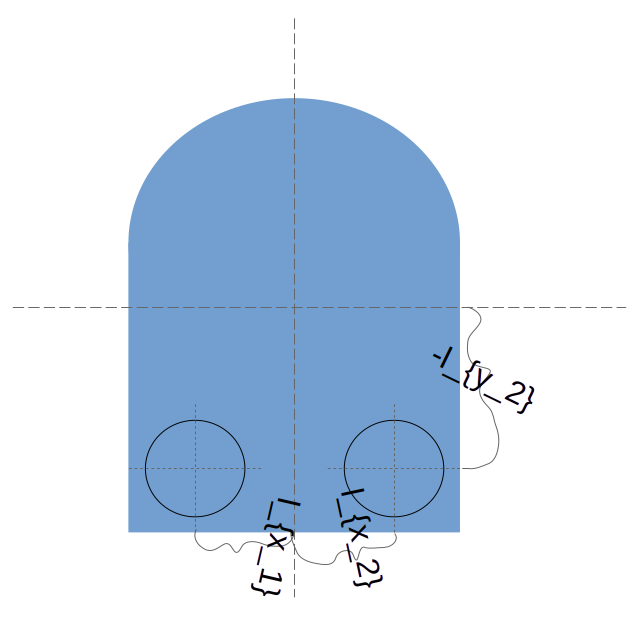
\includegraphics[width=0.9\textwidth]{thruster_position_sketch}
    \caption{Sketch of how the thruster position values in \cref{eq:transform_matrix} are found. The thruster configuration will be input to the allocator through a config file.}
    \label{fig:thruster_position_sketch}
\end{figure}

Since \(\tau\) and \(T\) are known, we can find \(f\) by performing a pseudoinverse on \(T\) leading us to the equation

\begin{equation}\label{eq:final_allocator}
f = T^\dagger \tau
\end{equation}

where \(T^\dagger\) is the pseudoinverse of \(T\).

This can also be written longform as

\begin{equation}\label{eq:long_allocator}
\begin{bmatrix}x_1 \\ y_1 \\ x_2 \\ y_2 \end{bmatrix} = T^\dagger \begin{bmatrix}X \\ Y \\ N\end{bmatrix}
\end{equation}

The full matrix for \(T^\dagger\) is omitted because the pseudoinverse of a non-square matrix tends to be large and ugly. It will only be handled by machine hands anyway, and as such doesn't matter right now.

The ROV has a built-in allocator which works well enough. The only issue with the ROV's allocator is that it's configured for a neutrally buoyant vessel. For this system we need to filter the vertical force component so the ROV only handles high-frequent/small-amplitude responses and the crane handles larger amplitudes and lower frequencies. This is also necessary because of elasticity in the lifting cable.

\section{Local control and physical response}
The vessel in this iteration has two thrusters. The ROV has a closed working solution and will not be considered here except for in the hypothetical. Each of these local controllers receive a two-component vector (or three-component in the case of the ROV) which instructs the controller what the desired thrust is. The azimuth thrusters on the USV are able to apply a force in one direction (parallel to the propeller axis), but they are able to vector this one-dimensional thrust using the azimuth ring.
